\lab{Introduction to SymPy}{Introduction to SymPy}

\objective{Most implementations of numerical algorithms focus on crunching, relating, or visualizing numerical data.
However, it is sometimes convenient or necessary to represent parts of an algorithm symbolically.
The SymPy module provides a way to do symbolic mathematics in Python, including algebra, differentiation, integration, and more.
In this lab, we introduce SymPy syntax and emphasize how to use symbolic algebra for numerical computing.}

\section*{Symbolic Variables and Expressions} % ===============================

Most variables in Python refer to a number, string, or data structure.
Doing computations on such variables results in more numbers, strings, or data structures.
A \emph{symbolic variable} is a variable that represents a mathematical symbol, such as $x$ or $\theta$, not a number or another kind of data.
Operating on symbolic variables results in an \emph{expression}, representative of an actual mathematical expression.
For example, if a symbolic variable \li{Y} refers to a mathematical variable $y$, the multiplication \li{3*Y} refers to the expression $3y$.
This is all done without assigning an actual numerical value to \li{Y}.

SymPy is Python's library for doing symbolic algebra and calculus.
It is typically imported with \li{import sympy as sy}, and symbolic variables are usually defined using \li{sy.symbols()}.
% Expressions can also be derived from a string using \li{sy.sympify()} or the shortcut \li{sy.S()}.
% \li{sy.Symbol()} can also be used to define a single variable, but will not be used in this lab for consistency.

\begin{lstlisting}
>>> import sympy as sy
>>> x0 = sy.symbols('x0')                   # Define a single variable.

# Define multiple symbolic variables simultaneously.
>>> x2, x3 = sy.symbols('x2, x3')           # Separate symbols by commas,
>>> m, a = sy.symbols('mass acceleration')  # by spaces,
>>> x, y, z = sy.symbols('x:z')             # or by colons.
>>> x4, x5, x6 = sy.symbols('x4:7')

# Combine symbolic variables to form expressions.
>>> expr = x**2 + x*y + 3*x*y + 4*y**3
>>> force = m * a
>>> print(expr, force, sep='\n')
x**2 + 4*x*y + 4*y**3
acceleration*mass
\end{lstlisting}
%
% # Create an expression from a string.
% >>> sy.S("x0**2+x1**3+x2")
% x0**2 + x1**3 + x2

% Pre-defined variables, including greek letters, can be imported from \li{sympy.abc}.
% To see a list of these variables, run \li{dir(sy.abc)} after \li{sy.abc} has been imported.

SymPy has its own version for each of the standard mathematical functions like $\sin(x)$, $\log(x)$, and $\sqrt{x}$, and includes predefined variables for special numbers such as $\pi$.
The naming conventions for most functions match NumPy, but some of the built-in constants are named slightly differently.
\[
\begin{array}{cl}
\text{Functions}
&
\begin{tabular}{c|c|c|c|c|c}
    $\sin(x)$ & $\arcsin(x)$ & $\sinh(x)$ & $e^x$ & $\log(x)$ & $\sqrt{x}$
    \\ \hline
    \li{sy.sin()} & \li{sy.asin()} & \li{sy.sinh()} & \li{sy.exp()} & \li{sy.log()} & \li{sy.sqrt()}
\end{tabular}
\\ \\
\text{Constants}
&
\begin{tabular}{c|c|c|c}
    $\pi$ & $e$ & $i = \sqrt{-1}$ & $\infty$
    \\ \hline
    \li{sy.pi} & \li{sy.E} & \li{sy.I} & \li{sy.oo}
\end{tabular}
\end{array}
\]
Other trigonometric functions like $\cos(x)$ follow the same naming conventions.
For more a complete list of SymPy functions, see \url{http://docs.sympy.org/latest/modules/functions/index.html}.

\begin{warn}
Always use SymPy functions and constants when creating expressions instead of using NumPy's functions and constants.
Later we will show how to make NumPy and SymPy cooperate.
\begin{lstlisting}
>>> import numpy as np

>>> x = sy.symbols('x')
>>> np.exp(x)                       # Try to use NumPy to represent e**x.
<<Traceback (most recent call last):
  File "<stdin>", line 1, in <module>
AttributeError: 'Symbol' object has no attribute 'exp'>>

>>> sy.exp(x)                       # Use SymPy's version instead.
<<exp(x)>>
\end{lstlisting}
\end{warn}

\begin{info}
SymPy defines its own numeric types for integers, floats, and rational numbers.
For example, the \li{sy.Rational} class is similar to the standard library's \li{fractions.Fraction} class, and should be used to represent fractions in SymPy expressions.

\begin{lstlisting}
>>> x = sy.symbols('x')
>>> (2/3) * sy.sin(x)               # 2/3 returns a float, not a rational.
0.666666666666667*sin(x)

>>> sy.Rational(2, 3) * sy.sin(x)   # Keep 2/3 symbolic.
2*sin(x)/3
\end{lstlisting}
Always be aware of which numeric types are being used in an expression.
Using rationals and integers where possible is important in simplifying expressions.
% To keep $\frac{2}{3}$ symbolic, use \li{sy.Rational(2,3)*sy.sin(x)} or \li{sy.Integer(2)/3*sy.sin(x)}.
\end{info}

\begin{problem} % Write a simple expression.
Write a function that returns the expression $\frac{2}{5} e^{x^2-y}\cosh(x+y) + \frac{3}{7}\log(xy+1)$ symbolically.
Make sure that the fractions remain symbolic.
\end{problem}

\subsection*{Sums and Products} % ---------------------------------------------

Expressions that can be written as a sum or a product can be constructed with \li{sy.summation()} or \li{sy.product()}, respectively.
Each of these functions accepts an expression that represents one term of the sum or product, then a tuple indicating the indexing variable and which values it should take on.
For example, the following code constructs the sum and product given below.
\[
\sum_{i=1}^{4} x + iy
\qquad\qquad
\prod_{i=0}^{5} x + iy
\]

\begin{lstlisting}
>>> x, y, i = sy.symbols('x y i')

>>> sy.summation(x + i*y, (i, 1, 4))    # Sum over i=1,2,3,4.
<<4*x + 10*y>>

>>> sy.product(x + i*y, (i, 0, 5))      # Multiply over i=0,1,2,3,4,5.
<<x*(x + y)*(x + 2*y)*(x + 3*y)*(x + 4*y)*(x + 5*y)>>
\end{lstlisting}

\subsection*{Simplifying Expressions} % ---------------------------------------

The expressions for the summation and product in the previous example are automatically simplified.
More complicated expressions can be simplified with one or more of the following functions.

\begin{table}[H]
\centering
\begin{tabular}{r|l}
Function & Description \\ \hline
% \li{sy.apart()} & Partial fraction decomposition. \\
\li{sy.cancel()} & Cancel common factors in the numerator and denominator. \\
% \li{sy.collect()} & Factor out all rational powers of a specified variable. \\
\li{sy.expand()} & Expand a factored expression. \\
\li{sy.factor()} & Factor an expanded expression. \\
% \li{powsimp()} & Combine powers with similar bases and exponents. \\
\li{sy.radsimp()} & Rationalize the denominator of an expression. \\
% \li{sy.ratsimp()} & Return the simplest form of the addition of two rational expressions. \\
% \li{seperate()} & Rewrite a power of products to a product of powers. \\
\li{sy.simplify()} & Simplify an expression.\\
% \li{together()} & Combine rational functions.\\
\li{sy.trigsimp()} & Simplify only the trigonometric parts of the expression. \\
\end{tabular}
\end{table}

\begin{lstlisting}
>>> x = sy.symbols('x')
>>> expr = (x**2 + 2*x + 1) / ((x+1)*((sy.sin(x)/sy.cos(x))**2 + 1))
>>> print(expr)
(x**2 + 2*x + 1)/((x + 1)*(sin(x)**2/cos(x)**2 + 1))

>>> sy.simplify(expr)
(x + 1)*cos(x)**2
\end{lstlisting}

The generic \li{sy.simplify()} tries to simplify an expression in any possible way.
This is often computationally expensive; using more specific simplifiers when possible reduces the cost.

\begin{lstlisting}
>>> expr = sy.product(x + i*y, (i, 0, 3))
>>> print(expr)
x*(x + y)*(x + 2*y)*(x + 3*y)

>>> expr_long = sy.expand(expr)         # Expand the product terms.
>>> print(expr_long)
x**4 + 6*x**3*y + 11*x**2*y**2 + 6*x*y**3

>>> expr_long /= (x + 3*y)
>>> print(expr_long)
(x**4 + 6*x**3*y + 11*x**2*y**2 + 6*x*y**3)/(x + 3*y)

>>> expr_short = sy.cancel(expr_long)   # Cancel out the denominator.
x**3 + 3*x**2*y + 2*x*y**2

>>> sy.factor(expr_short)               # Factor the result.
x*(x + y)*(x + 2*y)

# Simplify the trigonometric parts of an expression.
>>> sy.trigsimp(2*sy.sin(x)*sy.cos(x))
<<sin(2*x)>>
\end{lstlisting}

See \url{http://docs.sympy.org/latest/tutorial/simplification.html} for more examples.

\begin{warn}
% Keep the following in mind when simplifying expressions.
\begin{enumerate}
\item Simplifications return new expressions; they do not modify existing expressions in place.

\item The \li{==} operator compares two expressions for exact structural equality, not algebraic equivalence.
Simplify or expand expressions before comparing them with \li{==}.

\item Expressions containing floats may not simplify as expected.
Always use integers and SymPy rationals in expressions when appropriate.
\end{enumerate}

\begin{lstlisting}
>>> expr = 2*sy.sin(x)*sy.cos(x)
>>> sy.trigsimp(expr)
sin(2*x)
>> print(expr)
2*sin(x)*cos(x)                 # The original expression is unchanged.

>>> 2*sy.sin(x)*sy.cos(x) == sy.sin(2*x)
<<False>>                           # The two expression structures differ.

>>> sy.factor(x**2.0 - 1)
x**2.0 - 1                      # Factorization fails due to the 2.0.
\end{lstlisting}
\end{warn}

\begin{problem}
Write a function that computes and simplifies the following expression.
\[\prod_{i=1}^{5} \sum_{j=i}^{5}j(\sin(x)+\cos(x))\]
\end{problem}

\section*{Evaluating Expressions} % ===========================================

Every SymPy expression has a \li{subs()} method that substitutes one variable for another.
The result is usually still a symbolic expression, even if a numerical value is used in the substitution.
The \li{evalf()} method actually evaluates the expression numerically after all symbolic variables have been assigned a value.
Both of these methods can accept a dictionary to reassign multiple symbols simultaneously.

\begin{lstlisting}
>>> x,y = sy.symbols('x y')
>>> expr = sy.expand((x + y)**3)
>>> print(expr)
x**3 + 3*x**2*y + 3*x*y**2 + y**3

# Replace the symbolic variable y with the expression 2x.
>>> expr.subs(y, 2*x)
27*x**3

# Replace x with pi and y with 1.
>>> new_expr = expr.subs({x:sy.pi, y:1})
>>> print(new_expr)
1 + 3*pi + 3*pi**2 + pi**3
>>> new_expr.evalf()                # Numerically evaluate the expression.
71.0398678443373

# Evaluate the expression by providing values for each variable.
>>> expr.evalf(subs={x:1, y:2})
27.0000000000000
\end{lstlisting}

These operations are good for evaluating an expression at a single point, but it is typically more useful to turn the expression into a reusable numerical function.
To this end, \li{sy.lambdify()} takes in a symbolic variable (or list of variables) and an expression, then returns a callable function that corresponds to the expression.

\begin{lstlisting}
# Turn the expression sin(x)^2 into a function with x as the variable.
>>> f = sy.lambdify(x, sy.sin(x)**2)
>>> print(f(0), f(np.pi/2), f(np.pi), sep='  ')
0.0  1.0  1.4997597826618576e-32

# Lambdify a function of several variables.
>>> f = sy.lambdify((x,y), sy.sin(x)**2 + sy.cos(y)**2)
>>> print(f(0,1), f(1,0), f(np.pi, np.pi), sep='  ')
0.2919265817264289  1.708073418273571  1.0
\end{lstlisting}

By default, \li{sy.lambdify()} uses the \li{math} module to convert an expression to a function.
For example, \li{sy.sin()} is converted to \li{math.sin()}.
By providing \li{"numpy"} as an additional argument, \li{sy.lambdify()} replaces symbolic functions with their NumPy equivalents instead, so \li{sy.sin()} is converted to \li{np.sin()}.
This allows the resulting function to act element-wise on NumPy arrays, not just on single data points.

\begin{lstlisting}
>>> f = sy.lambdify(x, 2*sy.sin(2*x), "numpy")
>>> f(np.linspace(0, 2*np.pi, 9))   # Evaluate f() at many points.
array([  0.00000000e+00,   2.00000000e+00,   2.44929360e-16,
        -2.00000000e+00,  -4.89858720e-16,   2.00000000e+00,
         7.34788079e-16,  -2.00000000e+00,  -9.79717439e-16])
\end{lstlisting}

\begin{info}
It is almost always computationally cheaper to lambdify a function than to use substitutions.
According to the SymPy documentation, using \li{sy.lambdify()} to do numerical evaluations ``takes on the order of hundreds of nanoseconds, roughly two orders of magnitude faster than the \li{subs()} method.''

\begin{lstlisting}
<g<In [1]:>g> import sympy as sy
<g<In [2]:>g> import numpy as np

# Define a symbol, an expression, and points to plug into the expression.
<g<In [3]:>g> x = sy.symbols('x')
<g<In [4]:>g> expr = sy.tanh(x)
<g<In [5]:>g> points = np.random.random(10000)

# Time using evalf() on each of the random points.
<g<In [6]:>g> <p<%time>p> _ = [expr.subs(x, pt).evalf() for pt in points]
<<CPU times: user 5.29 s, sys: 40.3 ms, total: 5.33 s
Wall time: 5.36 s>>

# Lambdify the expression and time using the resulting function.
<g<In [7]:>g> f = sy.lambdify(x, expr)
<g<In [8]:>g> <p<%time>p> _ = [f(pt) for pt in points]
<<CPU times: user 5.39 ms, sys: 648 micros, total: 6.04 ms
Wall time: 7.75 ms>>      # About 1000 times faster than evalf().

# Lambdify the expression with NumPy and repeat the experiment.
<g<In [9]:>g> f = sy.lambdify(x, expr, "numpy")
<g<In [10]:>g> <p<%time>p> _ = f(points)
<<CPU times: user 381 micros, sys: 63 micros, total: 444 micros
Wall time: 282 micros>>   # About 10 times faster than regular lambdify.
\end{lstlisting}
\end{info}

\begin{problem}
The Maclaurin series up to order $N$ for $e^x$ is defined as follows.
\begin{equation}
e^x \approx \sum_{n=0}^N \frac{x^n}{n!}
\label{eq:sympy-maclaurin-exponential}
\end{equation}
Write a function that accepts an integer $N$.
Define an expression for (\ref{eq:sympy-maclaurin-exponential}), then substitute in $-y^2$ for $x$ to get a truncated Maclaurin series of $e^{-y^2}$.
Lambdify the resulting expression and plot the series on the domain $y\in[-2,2]$.
Plot $e^{-y^2}$ over the same domain for comparison.
\\(Hint: use \li{sy.factorial()} to compute the factorial.)

Call your function with increasing values of $N$ to check that the series converges correctly.
\end{problem}

\section*{Solving Symbolic Equations} % =======================================

A SymPy expression by itself is not an equation.
However, \li{sy.solve()} equates an expression with zero and solves for a specified variable.
In this way, SymPy can be used to solve equations.

\begin{lstlisting}
>>> x,y = sy.symbols('x y')

# Solve x^2 - 2x + 1 = 0 for x.
>>> sy.solve(x**2 - 2*x + 1, x)
[1]                                 # The result is a list of solutions.

# Solve x^2 - 1 = 0 for x.
>>> sy.solve(x**2 - 1, x)
[-1, 1]                             # This equation has two solutions.

# Solutions can also be expressions involving other variables.
>>> sy.solve(x/(y-x) + (x-y)/y, x)
[y*(-sqrt(5) + 3)/2, y*(sqrt(5) + 3)/2]
\end{lstlisting}

\begin{problem}
The following equation represents a rose curve in cartesian coordinates.
\begin{equation}
0 = 1 - \frac{(x^2 + y^2)^{7/2} + 18x^5 y - 60x^3 y^3 + 18xy^5}{(x^2 + y^2)^3}
\label{eq:prob-polar-parametric}
\end{equation}
The curve is not the image of a single function (such a function would fail the vertical line test), so the best way to plot it is to convert (\ref{eq:prob-polar-parametric}) to a pair of parametric equations that depend on the angle parameter $\theta$.

Construct an expression for the nonzero side of (\ref{eq:prob-polar-parametric}) and convert it to polar coordinates with the substitutions $x = r\cos(\theta)$ and $y = r\sin(\theta)$.
Simplify the result, then solve it for $r$.
There are two solutions due to the presence of an $r^2$ term; pick one and lambdify it to get a function $r(\theta)$.
Use this function to plot $x(\theta) = r(\theta)\cos(\theta)$ against $y(\theta) = r(\theta)\sin(\theta)$ for $\theta \in [0,2\pi]$.
\\(Hint: use \li{sy.Rational()} for the fractional exponent.)
\end{problem}

\subsection*{Linear Algebra} % ------------------------------------------------

Sympy can also solve systems of equations.
A system of linear equations $A\x = \b$ is solved in a slightly different way than in NumPy and SciPy: instead of defining the matrix $A$ and the vector $\b$ separately, define the augmented matrix $M = [A\mid\b]$ and call \li{sy.solve_linear_system()} on $M$.

SymPy matrices are defined with \li{sy.Matrix()}, with the same syntax as $2$-dimensional NumPy arrays.
For example, the following code solves the system given below.
\[
\begin{array}{rrrrrrr}
 x & + &   y & + &  z & = & 5 \\
2x & + &  4y & + & 3z & = & 2 \\
5x & + & 10y & + & 2z & = & 4
\end{array}
\]
\begin{lstlisting}
>>> x, y, z = sy.symbols('x y z')

# Define the augmented matrix M = [A|b].
>>> M = sy.Matrix([ [1,  1, 1, 5],
                    [2,  4, 3, 2],
                    [5, 10, 2, 4] ])

# Solve the system, providing symbolic variables to solve for.
>>> sy.solve_linear_system(M, x, y, z)
{x: 98/11, y: -45/11, z: 2/11}
\end{lstlisting}

SymPy matrices support the standard matrix operations of addition \li{+}, subtraction \li{-}, and multiplication \li{@}.
Additionally, SymPy matrices are equipped with many useful methods, some of which are listed below.
See \url{http://docs.sympy.org/latest/modules/matrices/matrices.html} for more methods and examples.

\begin{table}[H]
\centering
\begin{tabular}{r|l}
Method & Returns \\ \hline
% \li{applyfunc()} & Apply a function to every element of the matrix. \\
% \li{condition_number()} & The condition number. \\
\li{det()} & The determinant. \\
% \li{diagonalize()} & Diagonalize a matrix. \\
\li{eigenvals()} & The eigenvalues and their multiplicities. \\
\li{eigenvects()} & The eigenvectors and their corresponding eigenvalues. \\
\li{inv()} & The matrix inverse. \\
\li{is_nilpotent()} & \li{True} if the matrix is nilpotent. \\
% \li{multiply_elementwise()} & Multiply matrices elementwise. \\
\li{norm()} & The Frobenius, $\infty$, $1$, or $2$ norm. \\
\li{nullspace()} & The nullspace as a list of vectors. \\
\li{rref()} & The reduced row-echelon form. \\
\li{singular_values()} & The singular values. \\
\end{tabular}
\end{table}

\begin{warn}
The \li{*} operator performs matrix multiplication on SymPy matrices.
To perform element-wise multiplication, use the \li{multiply_elementwise()} method instead.
\end{warn}

\begin{problem}
Find the eigenvalues of the following matrix by solving for $\lambda$ in the characteristic equation $\det(A - \lambda I) = 0$.
\begin{align*}
A =
\left[\begin{array}{cccc}
x-y & x   & 0   \\
x   & x-y & x   \\
0   & x   & x-y \\
\end{array}\right]
\end{align*}
Also compute the eigenvectors by solving the linear system $A - \lambda I = \0$ for each eigenvalue $\lambda$.
Return a dictionary mapping the eigenvalues to their eigenvectors.
\\(Hint: the \li{nullspace()} method may be useful.)

Check that $A\v = \lambda\v$ for each eigenvalue-eigenvector pair $(\lambda, \v)$.
Compare your results to the \li{eigenvals()} and \li{eigenvects()} methods for SymPy matrices.
\end{problem}

\section*{Calculus} % =========================================================

SymPy is also equipped to perform standard calculus operations, including derivatives, integrals, and taking limits.
Like other elements of SymPy, calculus operations can be temporally expensive, but they give exact solutions whenever solutions exist.

\subsection*{Differentiation} % -----------------------------------------------

The command \li{sy.Derivative()} creates a closed form, unevaluated derivative of an expression.
This is like putting $\frac{d}{dx}$ in front of an expression without actually calculating the derivative symbolically.
The resulting expression has a \li{doit()} method that can be used to evaluate the actual derivative.
Equivalently, \li{sy.diff()} immediately takes the derivative of an expression.

Both \li{sy.Derivative()} and \li{sy.diff()} accept a single expression, then the variable or variables that the derivative is being taken with respect to.

\begin{lstlisting}
>>> x, y = sy.symbols('x y')
>>> f = sy.sin(y)*sy.cos(x)**2

# Make an expression for the derivative of f with respect to x.
>>> df = sy.Derivative(f, x)
>>> print(df)
Derivative(sin(y)*cos(x)**2, x)

>>> df.doit()                       # Perform the actual differentiation.
-2*sin(x)*sin(y)*cos(x)

# Alternatively, calculate the derivative of f in a single step.
>>> sy.diff(f, x)
-2*sin(x)*sin(y)*cos(x)

# Calculate the derivative with respect to x, then y, then x again.
>>> sy.diff(f, x, y, x)
2*(sin(x)**2 - cos(x)**2)*cos(y)    # Note this expression could be simplified.
\end{lstlisting}

\begin{problem} % Single-variable optimization with differentiation.
Let $f:\mathbb{R}\rightarrow\mathbb{R}$ be a smooth function.
A \emph{critical point} of $f$ is a number $x_0\in\mathbb{R}$ satisfying $f'(x_0) = 0$.
The second derivative test states that a critical point $x_0$ is a local minimum of $f$ if $f''(x_0) > 0$, or a local maximum of $f$ if $f''(x_0) < 0$ (if $f''(x_0) = 0$, the test is inconclusive.

Now consider the following polynomial.
\[
p(x) = 2x^6 - 51x^4 + 48x^3 + 312x^2 - 576x - 100
\]
Use SymPy to find all critical points of $p$ and classify each as a local minimum or a local maximum.
Plot $p(x)$ over $x\in[-5,5]$ and mark each of the minima in one color and the maxima in another color.
Return the collections of local minima and local maxima as sets.
\end{problem}

The \emph{Jacobian matrix} of a multivariable function $f:\mathbb{R}^n \rightarrow \mathbb{R}^m$ at a point $\x_0 \in \mathbb{R}^n$ is the $m \times n$ matrix $J$ whose entries are given by
\begin{equation*}
J_{ij} = \frac{\partial f_i}{\partial x_j}(\x_0).
\end{equation*}
For example, the Jacobian for a function $f:\mathbb{R}^3 \rightarrow \mathbb{R}^2$ is defined by
\[
J = \left[\begin{array}{c|c|c}
\arrayrulecolor{gray}
\frac{\partial f}{\partial x_1}&\frac{\partial f}{\partial x_2}&\frac{\partial f}{\partial x_3}
\end{array}\right]
=
\left[\begin{array}{ccc}
\frac{\partial f_1}{\partial x_1}&\frac{\partial f_1}{\partial x_2}&\frac{\partial f_1}{\partial x_3}
\\ \\
\frac{\partial f_2}{\partial x_1}&\frac{\partial f_2}{\partial x_2}&\frac{\partial f_2}{\partial x_3}
\end{array}\right],
\qquad
\text{where}
\qquad
f(\x) =
\left[\begin{array}{c}
f_1(\x) \\ f_2(\x)
\end{array}\right],
\quad
\x = \left[\begin{array}{c}
x_1 \\ x_2 \\ x_3
\end{array}\right].
\]

To calculate the Jacobian matrix of a multivariate function with SymPy, define that function as a symbolic matrix (\li{sy.Matrix()}) and use its \li{jacobian()} method.
The method requires a list of variables that prescribes the ordering of the differentiation.

\begin{lstlisting}
# Create a matrix of symbolic variables.
>>> r, t = sy.symbols('r theta')
>>> f = sy.Matrix([r*sy.cos(t), r*sy.sin(t)])

# Find the Jacobian matrix of f with respect to r and theta.
>>> J = f.jacobian([r,t])
>>> J
Matrix([
[cos(theta), -r*sin(theta)],
[sin(theta),  r*cos(theta)]])

# Evaluate the Jacobian matrix at the point (1, pi/2).
>>> J.subs({r:1, t:sy.pi/2})
Matrix([
[0, -1],
[1,  0]])

# Calculate the (symbolic) determinant of the Jacobian matrix.
>>> sy.simplify(J.det())
r
\end{lstlisting}

\subsection*{Integration} % ---------------------------------------------------

The function \li{sy.Integral()} creates an unevaluated integral expression.
This is like putting an integral sign in front of an expression without actually evaluating the integral symbolically or numerically.
The resulting expression has a \li{doit()} method that can be used to evaluate the actual integral.
Equivalently, \li{sy.integrate()} immediately integrates an expression.

Both \li{sy.Derivative()} and \li{sy.diff()} accept a single expression, then a tuple or tuples containing the variable of integration and, optionally, the bounds of integration.

\begin{lstlisting}
# Calculate the indefinite integral of sec(x).
>>> sy.integrate(sy.sec(x), x)
-log(sin(x) - 1)/2 + log(sin(x) + 1)/2

# Integrate cos(x)^2 from 0 to pi/2.
>>> sy.integrate(sy.cos(x)**2, (x,0,sy.pi/2))
pi/4

# Compute the integral of (y^2)(x^2) dx dy with x from 0 to 2, y from -1 to 1.
>>> sy.integrate(y**2 * x**2, (x,0,2), (y,-1,1))
16/9
\end{lstlisting}

\begin{problem}
% Many unpleasant integrals can be made tractable by a \emph{change of variables}, such as using polar, cylindrical, or spherical coordinates instead of the usual Cartesian system.
Let $f:\mathbb{R}^3\rightarrow\mathbb{R}$ be a smooth function.
The volume integral of $f$ over the sphere $S$ of radius $r$ can written in spherical coordinates as
\begin{align*}
\underset{S}{\iiint} f(x,y,z) dV = \int_0^\pi\int_0^{2\pi}\int_0^r f(h_1(\rho, \theta, \phi), h_2(\rho, \theta, \phi), h_3(\rho, \theta, \phi)) |\det(J)| \:d\rho\:d\theta\:d\phi,
\end{align*}
where $J$ is the Jacobian of the function $h:\mathbb{R}^3\rightarrow\mathbb{R}^3$ defined below.
\[
h(\rho, \theta, \phi) =
\left[\begin{array}{c}
h_1(\rho, \theta, \phi) \\
h_2(\rho, \theta, \phi) \\
h_3(\rho, \theta, \phi)
\end{array}\right]
=
\left[\begin{array}{c}
\rho\sin(\phi)\cos(\theta) \\
\rho\sin(\phi)\sin(\theta) \\
\rho\cos(\phi)
\end{array}\right]
\]
Calculate the volume integral of $f(x,y,z) = (x^2 + y^2 + z^2)^2$ over the sphere of radius $r$.
Lambdify the resulting expression (with $r$ as the independent variable) and plot the integral value for $r \in [0, 3]$.
In addition, return the value of the integral when $r=2$.
\\ (Hint: simplify the integrand before computing the integral.
In this case, $|\det(J)| = -\det(J)$.)

To check your answer, when $r=3$, the value of the integral is $\frac{8748}{7}\pi$.
\end{problem}

\begin{warn}
SymPy isn't perfect.
It solves some integrals incorrectly, simplifies some expressions poorly, and is significantly slower than numerical computations.
However, it is generally very useful for simplifying parts of an algorithm, getting exact answers, and handling tedious algebra quickly.
\end{warn}

\newpage

\section*{Additional Material} % ==============================================

\subsection*{Pretty Printing} % -----------------------------------------------

SymPy expressions, especially complicated ones, can be hard to read.
Calling \li{sy.init_printing()} changes the way that certain expressions are displayed to be more readable; in a Jupyter Notebook, the rendering is done with \LaTeX, as displayed below.
Furthermore, the function \li{sy.latex()} converts an expression into actual \LaTeX \ code for use in other settings.

\begin{center}
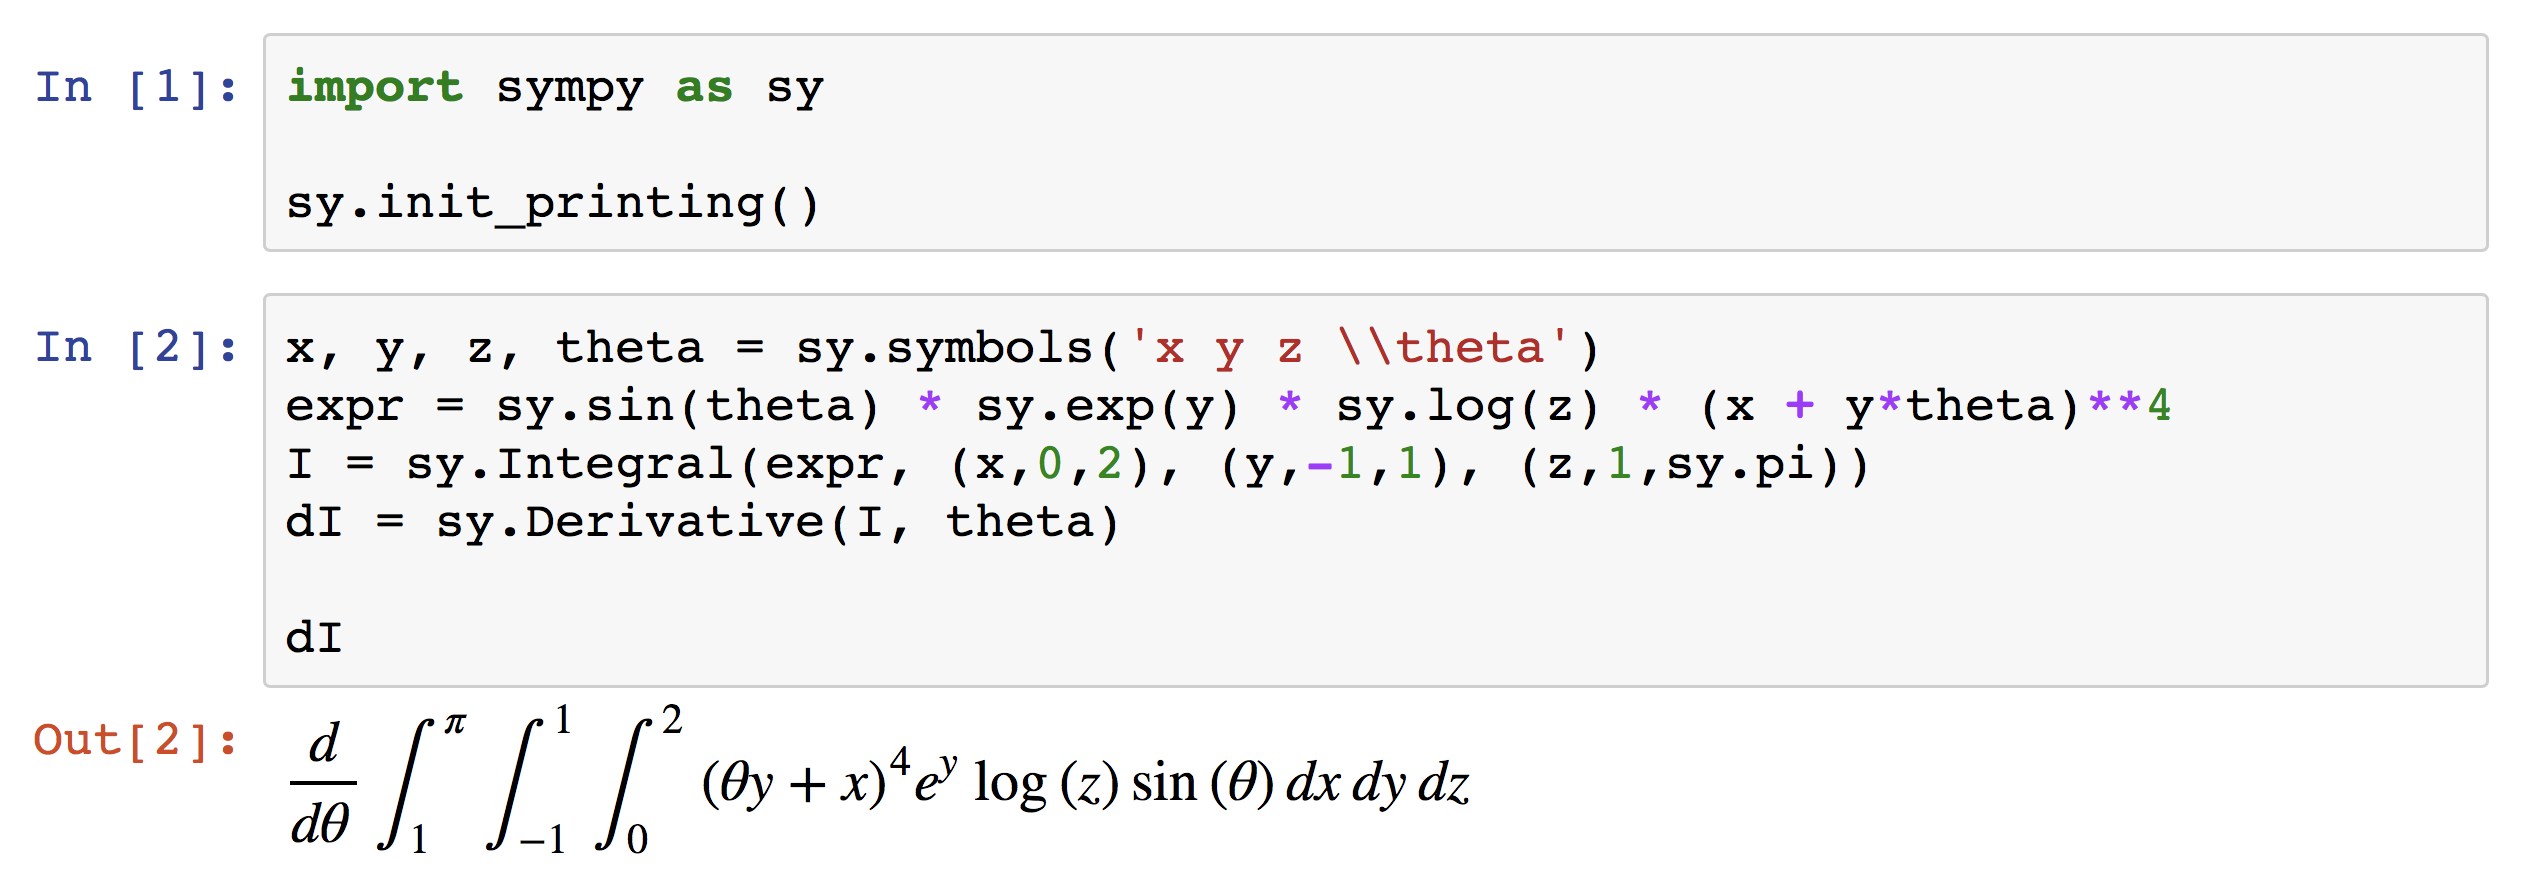
\includegraphics[width=\textwidth]{figures/pretty_printing.png}
\end{center}

% SymPy also has a simplified plotting wrapper around Matplotlib.
% See \url{http://docs.sympy.org/latest/modules/plotting.html} for further details.
% \begin{lstlisting}
% # Plot sin(x)e^x where x ranges from -3 to 3.
% >>> expr = sy.sin(x) * sy.exp(x)
% >>> sy.plot(expr, (x, -3, 3))
% \end{lstlisting}
%
% \begin{figure}[H]
% \includegraphics[width=.7\textwidth]{figures/plotting_wrapper.pdf}
% \end{figure}

\subsection*{Limits} % --------------------------------------------------------

Limits can be expressed, similar to derivatives or integrals, with \li{sy.Limit()}.
Alternatively, \li{sy.limit()} (lowercase) evaluates a limit directly.

\begin{lstlisting}
# Define the limit of a^(1/x) as x approaches infinity.
>>> a, x = sy.symbols('a x')
>>> sy.Limit(a**(1/x), x, sy.oo)
<<Limit(a**(1/x), x, oo, dir='-')>>

# Use the doit() method or sy.limit() to evaluate a limit.
>>> sy.limit((1+x)**(1/x), x, 0)
E

# Evaluate a limit as x approaches 0 from the negative direction.
>>> sy.limit(1/x, x, 0, '-')
-oo
\end{lstlisting}

Use limits instead of the \li{subs()} method when the value to be substituted is $\infty$ or is a singularity.

\begin{lstlisting}
>>> expr = x / 2**x
>>> expr.subs(x, sy.oo)
nan
>>> sy.limit(expr, x, sy.oo)
0
\end{lstlisting}

Refer to \url{http://docs.sympy.org/latest/tutorial/calculus.html} for SymPy's official documentation on calculus operations.

\begin{comment} % Too much additional material already.
\subsection*{Series Expansions} % ---------------------------------------------

Series can be depicted using the summation function, but SymPy also has built-in functions to depict them.
Expressions involving series can be created using \li{series()} as a function or as a method.
The function takes in the expression, variable, the point the series is centered at, and the order of the series.
The point the series is centered at defaults to zero and the order to six.

\begin{lstlisting}
# Find the terms in the series for cos(x) centered around x = 0 of order 6.
>>> sy.series(sy.cos(x),x)
1 - x**2/2 + x**4/24 + O(x**6)

# Center the series at x = pi of order 4.
>>> sy.series(sy.cos(x),x,sy.pi, 4)
-1 + (x - pi)**2/2 + O((x - pi)**4, (x,pi))

# Use removeO() to remove the order from the output.
>>> sy.series(sy.exp(sy.cos(x)),x,1,2).removeO()
-(x - 1)*exp(cos(1))*sin(1) + exp(cos(1))
\end{lstlisting}

Power series can be represented in SymPy with the ``Formal Power Series'' class.
When an \li{fps} object is created, it returns sequences of coefficients and powers, followed by the independent and then the common terms.
Use the \li{truncate()} or \li{polynomial()} methods to visualize individual terms of the series.
These methods input the highest order to be visualized and default to six.

\begin{lstlisting}
>>> f = sy.fps(sy.cos(x),x)
>>> f.truncate()
1 - x**2/2 + x**4/24 + O(x**6)
>>> f.polynomial()
x**4/24 - x**2/2 + 1
\end{lstlisting}

Further series features in SymPy include the computation of residues, laurent series and fourier series.
\end{comment}

\subsection*{Numerical Integration} % -----------------------------------------

Many integrals cannot be solved analytically.
% Additionally, the definite integral of a function may be undefined.
% If SymPy is unable to compute an integral, it returns an integral object.
As an alternative to the \li{doit()} method, the \li{as_sum()} method approximates the integral with a summation.
This method accepts the number of terms to use and a string indicating which approximation rule to use (\li{"left"}, \li{"right"}, \li{"midpoint"}, or \li{"trapezoid"}).

\begin{lstlisting}
>>> x = sy.symbols('x')

# Try integrating e^(x^2) from 0 to pi.
>>> I = sy.Integral(sy.exp(x**2), (x,0,sy.pi))
>>> I.doit()
sqrt(pi)*erfi(pi)/2                 # The result is not very helpful.

# Instead, approximate the integral with a sum.
>>> I.as_sum(10, 'left').evalf()
1162.85031639195
\end{lstlisting}

% In addition, SymPy includes several integral transforms, such as the Laplace, Fourier, sine, and cosine transforms.
% It can also do several types of integrals, such as line integrals.
See \url{http://docs.sympy.org/latest/modules/integrals/integrals.html} for more documentation on integration with SymPy.

\subsection*{Differential Equations} % ----------------------------------------

SymPy can be used to solve both ordinary and partial differential equations.
The documentation for working with PDE functions is at \url{http://docs.sympy.org/dev/modules/solvers/pde.html}

The general form of a first-order differential equation is $\frac{dx}{dt} = f(x(t),t)$.
To represent the unknown function $x(t)$, use \li{sy.Function()}.
Just as \li{sy.solve()} is used to solve an expression for a given \textbf{variable}, \li{sy.dsolve()} solves an ODE for a particular \textbf{function}.
When there are multiple solutions, \li{sy.dsolve()} returns a list; when arbitrary constants are involved they are given as \li{C1}, \li{C2}, and so on.
Use \li{sy.checkodesol()} to check that a function is a solution to a differential equation.

\begin{lstlisting}
>>> t = sy.symbols('t')
>>> x = sy.Function('x')

# Solve the equation x''(t) - 2x'(t) + x(t) = sin(t).
>>> ode = x(t).diff(t, t) - 2*x(t).diff(t) + x(t) - sy.sin(t)
>>> sy.dsolve(ode, x(t))
Eq(x(t), (C1 + C2*t)*exp(t) + cos(t)/2) # C1 and C2 are arbitrary constants.
\end{lstlisting}

Since there are many types of ODEs, \li{sy.dsolve()} may also take a hint indicating what solving strategy to use.
See \li{sy.ode.allhints} for a list of possible hints, or use \li{sy.classify_ode()} to see the list of hints that may apply to a particular equation.

% Old problem.
\begin{comment}
\begin{problem}
Return the solution to the following differential equation.
\begin{equation*}
 y_{xxx} + 3y_{xx} + 3y_{x} + y = x^{5}e^x + x^{4}\sin\left(x\right) + x^{3}\cos\left(3x\right)
\end{equation*}

Check the result $y(x)$ by plugging it back into an expression where one side of the equation is subtracted to another.
Use the \li{doit()} and \li{simplify()} methods to ensure that the new expression simplifies to $0$.
\end{problem}
\end{comment}
